\documentclass[runningheads]{llncs}

\usepackage[T1]{fontenc}
\usepackage{graphicx}
\usepackage{booktabs}
\usepackage{tikz}
\usepackage{pgfplots}
\usepackage{textcomp}
\pgfplotsset{width=15cm,compat=1.14}
\usepgfplotslibrary{dateplot}
\usetikzlibrary{plotmarks}

% If you use the hyperref package, please uncomment the following two lines
% to display URLs in blue roman font according to Springer's eBook style:
\usepackage{hyperref}

\usepackage{color}
\renewcommand\UrlFont{\color{blue}\rmfamily}
\urlstyle{rm}


\begin{document}

\title{A Model for Designing the Electoral Constuencies in Ireland}

\author{Barry O'Sullivan  \and Luis Quesada \and  Helmut Simonis \and Grace Tacadao}

\authorrunning{}

\institute{Insight SFI Centre for Data Analytics\\School for Computer Science and Information Technology\\University College Cork\\Cork Ireland\\
\email{helmut.simonis@insight-centre.org}\\
}

\maketitle              

\begin{abstract}

\keywords{Election Districting \and Constituencies \and Clustering}
\end{abstract}



\section{Introduction}
\label{sec:introduction}


\section{Problem Description and Related Work}
\label{sec:problem}

Different from many combinatorial optimization problems encountered in industry, the defining constraints for the election districting problems are well defined by law. 

We quote from Article 16 of the \emph{Irish Constitution}~\cite{Ireland2020}:
\begin{quote}
2\textdegree The number of members shall from time to time be fixed by law, but the total number of members of Dáil Éireann shall not be fixed at less than one member for each thirty thousand of the population, or at more than one member for each twenty thousand of the population.

3\textdegree The ratio between the number of members to be elected at any time for each constituency and the population of each constituency, as ascertained at the last preceding census, shall, so far as it is practicable, be the same throughout the country.

6\textdegree No law shall be enacted whereby the number of members to be returned for any constituency shall be less than three.
\end{quote}

More details about the creation of the constituencies is given in the ~\emph{Electoral Reform Act} of 2022~\cite{Ireland2022}, which in particular defines the following constraints in Section 57 (2):

\begin{quote}
(a) the total number of members of Dáil Éireann, subject to Article 16.2.2 of the Constitution, shall be not less than 171 and not more than 181;

(b) each constituency shall return 3, 4 or 5 members;

(c) the breaching of county boundaries shall be avoided as far as practicable;

(d) each constituency shall be composed of contiguous areas;

(e) there shall be regard to geographic considerations including significant physical features and the extent of and the density of population in each constituency;

(f) subject to this section, the Commission shall endeavour to maintain continuity in relation to the arrangement of constituencies.
\end{quote}


The \emph{Electoral Commission} was tasked with producing a proposal for the Constituency Review, the current draft proposal is described in~\cite{ElectoralCommission2023}. It describes the proposed revision of the constituencies for elections for Dáil Éireann, which we use for a baseline comparison, and for the simpler Irish constituency layout for the European Parliament, which we will not discuss in this paper.

In their terms of reference (page 18 of~\cite{ElectoralCommission2023}), the Commission extended (c) above as
\begin{quote}
the breaching of county boundaries shall be avoided as far as practicable (shall be deemed not to include a reference to the boundary of a city or any boundary between any two of the counties of Dún Laoghaire-Rathdown, Fingal and South Dublin);
\end{quote}
This means that the constituencies inside the Dublin area are not affected by the country borders, we follow this decision in our model, by treating Dublin as a single "county".  

While the solution given in~\cite{ElectoralCommission2023} is largely based on the existing electoral districts, it is important to note that in the solution given changes to a number of electoral districts are required (for example on page 127 for Cork North-Central). To achieve comparable results our solution may require similar changes.

As the Irish election system is quite different from many other countries, results on election districting~\cite{Almeida2022} are not directly transferable to the Irish situation. Only~\cite{Kotthoff2015} directly addresses the Irish scenario. Their model tries to allocate electoral districts to constituencies, satisfying the size limits imposed by law. To deal with the contiguity constraint, they use a constraint model based on the global \emph{tree} constraint~\cite{Beldiceanu2005} which ensures that all districts allocated to a constituency form one contiguous area. The model suffers from scalability issues, and only a partial solution for Galway is presented in the paper, with an execution time of 100 hours quoted on a multi-core computer. 



\section{Model}
\label{sec:model}

In this section we describe our top-level model of deciding how many constituencies of which size should be created in each county, and which transfer of areas between neighbouring counties should be considered to achieve the best compromise between the total number of seats considered, balancing the size of the constituencies, respecting the county boundaries, and creating constituencies with a mix of different sizes. Different stakeholders will want to weight the elements of this objective in different ways, we show that by stating additional constraints different parts of the overall solution space can be explored.

\subsection{Constants}

We use the set $I$ of all counties in the country, and use $i$ as an index. We consider the set $J$ of different constituency types, and use $j$ as an index. In the current Irish case there are three constituency types, with resp. three, four and five seats per constituency. Additional types may be considered for evaluation.

We use the following constant values in the model, some are defined as data, while others can be chosen as parameters or cost factors for a specific run. 

\begin{description}
\item[$n$] total population
\item[$lb$] lower bound on number of persons per seat, defined as 20,000 in constitution
\item[$ub$] upper bound on number of persons per seat, defined as 30,000 in constitution
\item[$k$] total number of seats, can be selected between $n/lb$ and $n/ub$ 
\item[$a$] average size of one seat, e.g. $n/k$
\item[$\Delta$] maximum allowed variation of the actual size of a seat, i.e. the number of persons represented by each seat must fall in the interval $[a-\Delta,a+\Delta]$ 
\item[$p_{i}$] population of county $i$
\item[$s_{j}$] number of seats in a constituency of type $j$
\item[$c_{i_1i_2}$] Boolean value, true iff counties $i_1$ and $i_2$ are neighbours 
\item[$\alpha$] cost per cross-border transfer
\item[$\beta$] cost per person assigned to a constituency outside their home county
\item[$\gamma_{j}$] cost of a constituency of type $j$
\end{description}

\subsection{Variables}

The main decision variables of the model are used for two purposes. The $x_{ij}$ variables indicate how many constituencies of type $j$ we create in county $i$. The variables $y_{i_1i_2}$ and $z_{i_1i_2}$ consider the reallocation of persons living in county $i_1$ to a constituency in county $i_2$. The $y$ variables are zero/one decision variables, indicating if a transfer is required at all, while the $z$ continuous variables count the number of persons re-allocated. We use auxiliary integer variables $u_{j}$ to constrain or count the number of constituencies of a type $j$ at a national level. 

\begin{description}
\item[$x_{ij}$] non-negative integer variable stating how many constituencies of size $j$ we create in county $i$
\item[$y_{i_1i_2}$] zero-one integer variable stating whether we assign population in county $i_{1}$ to a constituency defined in county $i_{2}$. The transfer only exists if counties $i_{1}$ and $i_{2}$ are neighbours.
\item[$z_{i_1i_2}$] non negative variable stating how many people we transfer from county $i_{1}$ to county $i_{2}$. $p_{i_1}$ is an upper bound for this variable. In a first version of the model we assume that any specific number of persons can be transferred, possibly requiring modifications of electoral districts. 
\item[$u_{j}$] the total number of constituencies of size $j$
\end{description}

\subsection{Constraints}

The total number of seats allocated to constituencies must be equal to the total number of seats given.
\begin{equation}
\sum_{i \in I} \sum_{j \in J} x_{ij}s_{j} = k
\end{equation}

The number of constituencies of each type $j$ is equal to the sum of constituencies of that type in all counties.
\begin{equation}
\forall_{j \in J}:\quad \sum_{i \in I} x_{ij} = u_{j}
\end{equation}

The effective population of a county $i$ (the population itself plus all transfers into the county minus all transfers out of the county) must be covered by the number of assigned seats of the county. A seat must at least represent $a-\Delta$ and at most $a+\Delta$ persons.
\begin{equation}
\forall_{i \in I}:\quad (a-\Delta)\sum_{j \in J} x_{ij}s_{j} \leq p_{i}+\sum_{i_1 \in I} z_{i_1i} - \sum_{i_2 \in I} z_{ii_2}\leq (a+\Delta)\sum_{j \in J} x_{ij}s_{j}
\end{equation}
Note that this form of the constraint assumes that we can split the total population in a county between the different constituencies exactly proportional to the number of seats allocated. This may require some changes to the electoral districts to balance the numbers.

The decision variable for a inter-country transfer is linked to the counting variable for the same transfer by a \emph{bigM} constraint. If the decision variable is zero, then the counting variable must also be zero. Inversely, if the count is greater than zero, then the decision variable must be one.
\begin{equation}
\forall_{i_1,i_2 \in I}:\quad z_{i_1i_2} \leq p_{i_1}y_{i_1i_2} 
\end{equation}

The total number of persons assigned to any constituency outside their county $i$ is limited by the population of the county. This value is reached if no constituency is allocated to the county at all.
\begin{equation}
\forall_{i \in I}:\quad \sum_{i_1 \in I} z_{ii_1} \leq p_{i}
\end{equation}

For any pair of neighbouring counties, we can only transfer population in one direction, 
\begin{equation}
\forall_{i_1,i_2 \in I}:\quad y_{i_1i_2} + y_{i_2i_1} \leq 1
\end{equation}

We can only have a transfer between neighbouring counties, e.g. transfers between counties that are not neighbours are not allowed.
\begin{equation}
\forall_{i_1,i_2 \in I}:\quad \neg c_{i_1i_2} \Rightarrow (y_{i_1i_2}  = 0)
\end{equation}

If we want to ensure that no seat represents more than $ub$ persons, we can enforce an additional inequality stating that the effective number of persons in a county must not exceed the $ub$ value per seat allocated to the county. 
\begin{equation}
\forall_{i \in I}:\quad p_{i}+\sum_{i_1 \in I} z_{i_1i} - \sum_{i_2 \in I} z_{ii_2}\leq ub\sum_{j \in J} x_{ij}s_{j}
\end{equation}


\subsection{Objective}

We consider the following elements of the objective of the problem. Different stakeholder may consider only some of the objective terms, or assign different weights to the cost terms.

\begin{itemize}
\item The actual variance of the number of population per assigned seat in each constituency.
\item The number of county border breaches, where part of a county is assigned to a constituency place in a neighbouring county
\item The total size of the population assigned to a constituency spanning multiple counties
\item The number of constituencies of different sizes, which can vary between three and five seats per constituency. Different stakeholders may prefer more smaller constituencies, or more of the larger ones. 
\end{itemize}

The objective function for the problem is then defined as 
\begin{equation}
\min \alpha \sum_{i_1,i_2 \in I} y_{i_1i_2} + \beta \sum_{i_1,i_2 \in I} z_{i_1i_2} + \sum_{j \in J} \gamma_{j}u_{j}
\end{equation}

\subsection{Performance Indicators}

In order to compare and evaluate solutions, we compute different key performance indicators (KPIs) from the solutions found. We use them to compare solutions obtained for different input parameter values and constraints selected.

\begin{table}[htbp]
\caption{\label{tab:kpis}Key Performance Indicator Definition} 
\begin{tabular}{llp{7cm}}\toprule
Symbol & Definition & Explanation\\ \midrule
$k$ & parameter & total number of seats allocated\\
$\Delta$ & parameter & maximum $\pm$ range of persons per seat\\
$x$ & $\sum_{i \in I, j \in J} x_{ij}$ & total number of constituencies allocated \\
$t$ & k/x & average number of seats in the constituencies \\
$a$ & $n/k$ &average number of persons represented by seat\\
$y$& $\sum_{i_1,i_2 \in I} y_{i_1i_2}$& total number of inter-county allocations of non-zero size\\
$z$& $\sum_{i_1,i_2 \in I} z_{i_1i_2}$& total number of persons allocated to constituencies outside their home county\\
$q_{i}$ & $p_{i}+\sum_{i_1 \in I} z_{i_1i} - \sum_{i_2 \in I} z_{ii_2}$ & effective population for county $i$\\
$f_{i}$ & $\sum_{j \in J} x_{ij}s_{j}$ & number of seats allocated to county $i$ \\
$e_{i}$ & $q_{i}/f_{i}$ & actual number of persons per seat for county $i$\\
$\bar{e}$ & $\max_{i \in I} e_{i}$ & largest number of persons represented by any seat \\
$\underbar{e}$ & $\min_{i \in I} e_{i}$ & smallest number of persons represented by any seat\\ 
$r$ & $100.0(\bar{e}-\underbar{e})/a$ & representation range percentage\\
$w_{j}$ & $100.0u_{j}/x$ & percentage of constituencies of type $j$ \\
$$ & $$ & variance of voting power per person \\
\bottomrule
\end{tabular}
\end{table}


\subsection{Experiments}
\subsection{Data}
We use the population data for Ireland from the last Census in 2022~\cite{CSO2022}, Table F1004A on the CSO website provides county level counts, we aggregate the values for Dublin from the counties involved. Note that we treat Cork city and Galway city as individual entries separate from the corresponding counties. 

\subsection{Baseline Results}

We use the solution proposed in~\cite{ElectoralCommission2023} as a baseline. Figure~\ref{fig:baseline} shows the proposed constituency structure, based on a total population of 5,149,139 and 174 seats for the next Dáil, an increase of 14 over the current parliament. The solution creates 43 constituencies (13 of size three, 15 each of sizes four and five). Six inter-county transfers are suggested, affecting xxx persons. The percentage variance in sizes varies from -8.13\% to 8.08\%, for a total range of 16.21\%. Compared to the current constituency structure, 82\% of all constituencies will be changed.

\begin{figure}[htbp]
\caption{\label{fig:baseline} Baseline Solution from~\cite{ElectoralCommission2023}}
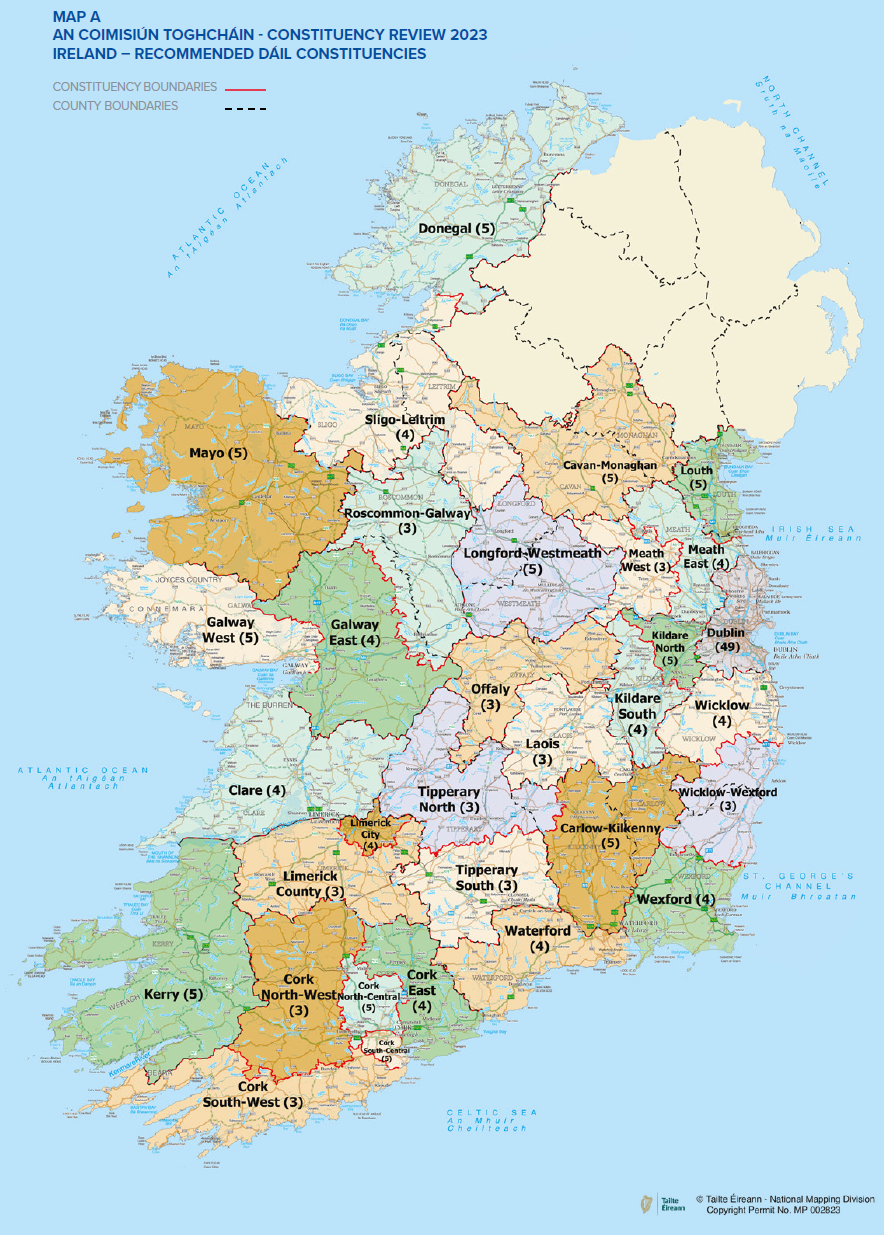
\includegraphics[width=\textwidth]{images/baseline}
\end{figure}

Table~\ref{tab:baselinetransfer} shows the inter-county transfers extracted manually from the descriptions in~\cite{ElectoralCommission2023}. Note that we find more transfers than stated in the document.

\begin{table}[htbp]
\caption{\label{tab:baselinetransfer}Inter-County Transfers in Baseline Solution}
\begin{tabular}{lllrr}\toprule
Constituency & From & To & Volume & Percentage of Total From\\ \midrule 
Sligo-Leitrim & Leitrim & Sligo & 35,199 & 100.00\%\\
Roscommon-Galway & Galway & Roscommon & 14,468 & \\
Cavan-Monaghan & Monaghan & Cavan & 65,288& 100.00\%\\
Louth & Meath & Louth & 16,403& \\
Tipperary-North & Kilkenny & Tipperary & 6,431& \\
Longford-Westmeath & Longford & Westmeath & 46,751& 100.00\%\\
Carlow-Kilkenny & Carlow & Kilkenny & 61,968& 100.00\%\\
Wicklow-Wexford & Wicklow & Wexford & 35,708& \\
\midrule
Total & & & & n/a\\
\bottomrule
\end{tabular}
\end{table}



\section{Results}
\label{sec:results}

\section{Conclusion}
\label{sec:conclusion}



% ---- Bibliography ----
%
% BibTeX users should specify bibliography style 'splncs04'.
% References will then be sorted and formatted in the correct style.
%

\bibliographystyle{splncs04}
\bibliography{election}

\appendix
\clearpage
\section{County Population Based on 2022 Census}
Table~\ref{tab:countypop} shows the population data used in~\cite{ElectoralCommission2023} for the counties considered. Our program uses identical data obtained directly from the CSO website~\cite{CSO2022} in machine readable form.

\begin{table}[htbp]
\caption{\label{tab:countypop}County Population}
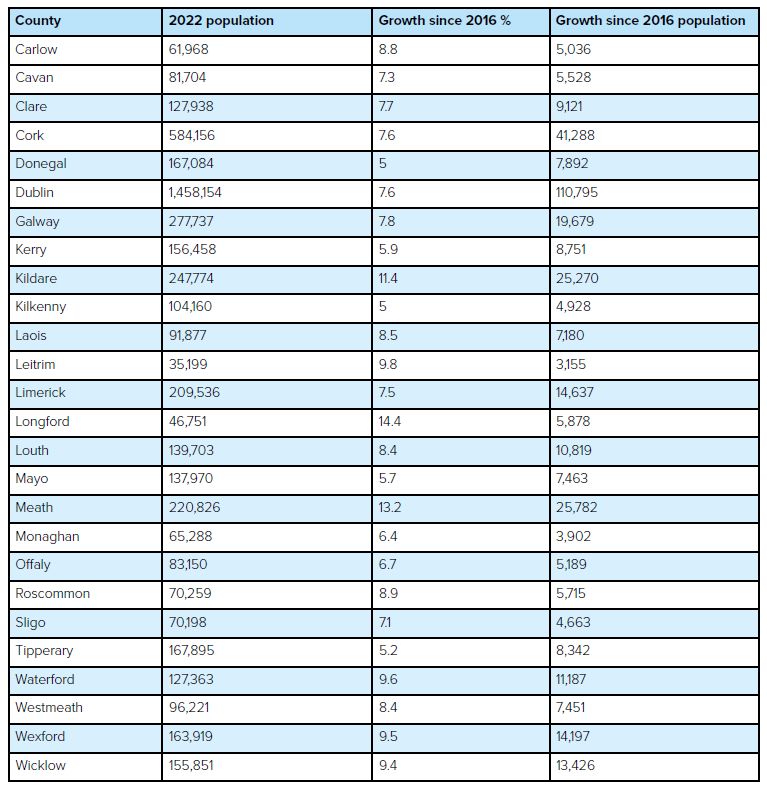
\includegraphics[width=\textwidth]{images/countypop}
\end{table}

\section{Baseline Constituencies}

Table~\ref{tab:baselinetable} shows a table of the 43 constituencies proposed in~\cite{ElectoralCommission2023} for a total of 174 seats, with their individual number of seats, allocated population, persons per TD, and variance against the national average of 29,593. The largest negative variance of -8.13\% occurs in Kildare South, the largest positive variance of 8.08\% occurs for the Clare constituency. Note that 17 of the proposed constituencies are assigned more than 30,000 persons per TD.

\begin{table}[htbp]
\caption{\label{tab:baselinetable}Baseline Constituency Structure}
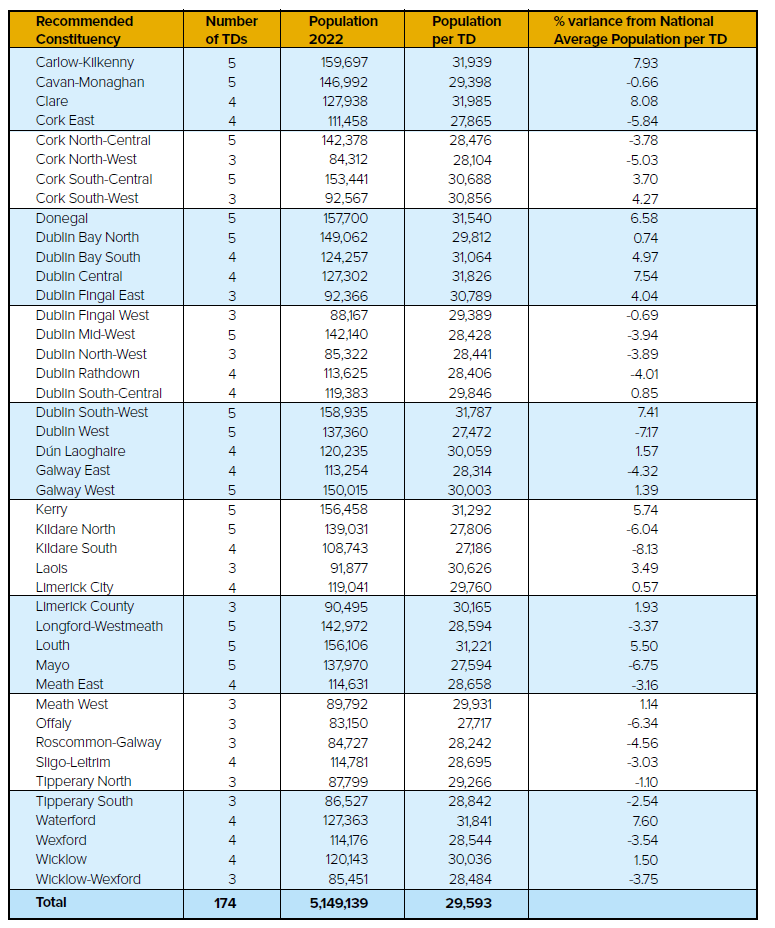
\includegraphics[width=\textwidth]{images/baselinetable}
\end{table}

\end{document}
